\section{Habib Abdul Rasyid}
\subsection{ Apa itu fungsi device manager di windows dan folder /dev di linux}
Device Manager adalah Panel Kontrol dalam sistem operasi Microsoft Windows. Ini memungkinkan pengguna untuk melihat dan mengontrol perangkat keras yang terpasang pada komputer. Ketika beberapa bagian perangkat keras tidak berfungsi, perangkat keras yang terkait akan disorot oleh pengguna. Daftar perangkat keras dapat disortir berdasarkan berbagai kriteria.
Untuk setiap perangkat, pengguna dapat:
\begin{itemize}
     \item Menyediakan driver perangkat sesuai dengan Model Driver Windows
     \item Aktifkan atau nonaktifkan perangkat
     \item Beri tahu Windows untuk mengabaikan perangkat yang tidak berfungsi
     \item Lihat sifat teknis lainnya
\end{itemize}
Device Manager diperkenalkan dengan Windows 95 dan kemudian ditambahkan ke Windows 2000. Dalam versi berbasis NT, ini dimasukkan sebagai snap-in Konsol Manajemen Microsoft.\newline

/ dev adalah lokasi file khusus atau perangkat. Ini adalah direktori yang sangat menarik yang menyoroti satu aspek penting dari sistem file Linux - semuanya adalah file atau direktori.


\subsection{Jelaskan langkah-langkah instalasi driver dari Arduino}
Berikut ini merupakan langkah-langkah untuk melakukan instalasi driver Arduino
\begin{itemize}
	\item Pertama-tama, pasang board arduino pada pc/Laptop. Kemudian tunggu sampai muncul pop up install driver, jika bermasalah lanjut ke step berikutnya
	\item buka Device Manager 
	\item Pilih unknown device
	\item klik kanan pada unknown device , dan pilih update software
	\item Masuk ke directory arduino untuk memilih folder drivernya
	\item klik Next
	\item Jika telah berhasil, maka tulisannya adalah Successfully
\end{itemize}

\subsection{Jelaskan bagaimana cara membaca baudrate dan port dari komputer yang sudah terinstal driver}
Berikut ini merupakan cara membaca baudrate dan port dari komputer yang sudah terinstal driver :
\begin{itemize}
	\item Pastikan Arduino terhubung dengan PC
	\item Kemudian buka software arduino pada pc
	\item Setelah itu, pilih tipe sesuai dengan yang digunakan
	\item Kemudian memilih serial port yang aktif  
	\item Klik Upload untuk memasukkan program ke arduino
	\item Setelah proses upload selesai, buka fitur serial monitor
	\item Lalu sesuaikan Baudrate pada serial monitor dengan Baudrate yang terdapat pada program
\end{itemize}

\subsection{Jelaskan sejarah library pyserial}
Pyserial berfungsi untuk merangkum akses untuk port serial. Pyserial menyediakan backends untuk Python yang berjalan pada sistem operasi Windows, Linux, BSD (mungkin sistem yang mendukung POSIX), Jython dan IronPython (.NET dan Mono). Modul bernama "serial" secara otomatis memilih backend yang sesuai. Antarmuka berbasis kelas yang sama pada semua platform yang didukung.
Akses ke pengaturan port melalui properti Python.
File seperti API dengan "read" dan "write" ("readline" dll. Juga didukung).
File-file dalam paket ini adalah 100 persen Python murni.
Port diatur untuk transmisi biner. Tidak ada stripping byte NULL, terjemahan CR-LF dll. (Yang berkali-kali diaktifkan untuk POSIX.)

\subsection{Jelaskan fungsi-fungsi apa saja yang dipakai dari library pyserial}
Serial – fungsi ini untuk membuka port serial
Read(size) – untuk membaca jumlah byte dari port serial
Write(data) – untuk menulis data lewat port serial
Close() – ini untuk menutup port serial 
Readline() – untuk membaca string dari port serial

\subsection{Jelaskan kenapa butuh perulangan dalam tidak butuh perulangan dalam membaca serial}
Perualangan berfungsi menyuruh komputer melakukan sesuatu secara berulang-ulang. Terdapat dua jenis perualangan dalam bahasa pemrograman python, yaitu perulangan dengan for dan while.
Perulangan for disebut counted loop  atau perulangan yang terhitung, sementara perulangan while disebut uncounted loop atau perulangan yang tak terhitung. Perulangan diperlukan agar dapat membaca data secara berulang kali sehingga data yang muncul lebih dari satu.  Sedangkan apabila tidak memakai perulangan maka data akan terbaca satu kali saja.

\subsection{Jelaskan bagaimana cara membuat fungsi yang mengunakan pyserial}
Berikut merupakan contoh penggunaan fungsi yang menggunakan pyserial
\lstinputlisting[firstline=5, lastline=15]{src/5/Teori/T1174002.py}

\subsection{Plagiarisme}
\begin{figure}[h]
\centering
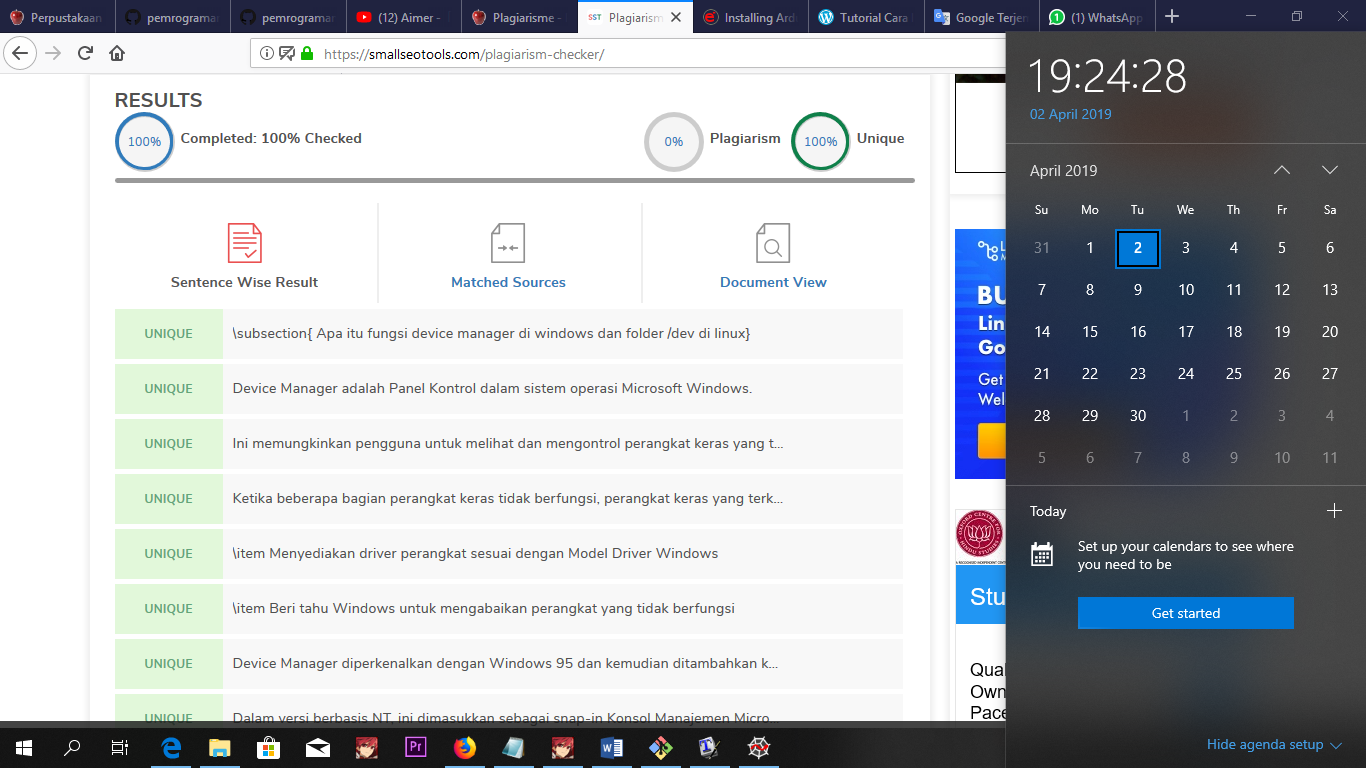
\includegraphics[scale=0.2]{figures/5/Teori/1174002/plagiat.png}
\caption{Plagiarisme}
\label{fig:plagiat}
\end{figure}

\section{Nico Ekklesia Sembiring}
\subsection{Apa itu fungsi device manager di windows dan folder /dev di linux}
berikut ini adalah fungsi device manager :
\begin{itemize}
	\item untuk menunjukkan status hardwarenya
	\item untuk menunjukkan informasi hardware secara detail
	\item Melakukan kelola driver pada hardware, seperti melakukan instalasi, uninstal, rollback, dan masalah lain yang berkaitan dengan driver.
	\item Melakukan identifikasi terhadap konflik yang terjadi pada hardware
\end{itemize}

Sedangkan folder /dev berisi file dari perangkat (Device), seperti device blok dan juga device karakter. Di dalam /dev minimal harus terdapat file biner MAKEDEV untuk dapat membuat device ini secara manual.
Di dalam sistem operasi Linux, setiap device yang tersambung akan dideteksi sebagai files, dan di dalam direktori /dev tersebut file-file khusus yang mempresentasikan perangkat tersimpan.

\subsection{Jelaskan langkah-langkah instalasi driver dari Arduino}
Berikut ini merupakan langkah-langkah untuk melakukan instalasi driver Arduino
\begin{itemize}
	\item Pertama-tama, pasang board arduino pada pc. Kemudian tunggu sampai windows mencoba menginstal sendiri. jika gagal, lanjutkan ke step selanjutnya
	\item buka Device Manager 
	\item Cari nama arduino atau "Unknown Device"
	\item klik kanan pada unknown device , dan pilih update software
	\item Cari folder instalan software arduino
	\item klik Next
	\item Jika telah berhasil, maka proses instal driver sudah selesai
\end{itemize}

\subsection{Jelaskan bagaimana cara membaca baudrate dan port dari komputer yang sudah terinstal driver}
Berikut ini merupakan cara membaca baudrate dan port dari komputer yang sudah terinstal driver :
\begin{itemize}
	\item Sambungkan port USB arduino dengan port USB pc
	\item Kemudian buka software arduino pada pc
	\item Setelah itu, pilih tipe arduino yang digunakan
	\item Kemudian memilih serial port yang aktif  
	\item Selanjutnya untuk memasukkan program pada arduino, klik tombol upload
	\item Setelah proses upload selesai, buka fitur serial monitor
	\item Lalu sesuaikan Baudrate pada serial monitor dengan Baudrate yang terdapat pada program
\end{itemize}

\subsection{Jelaskan sejarah library pyserial}
Pyserial berguna untuk merangkum akses untuk port serial. Pyserial menyediakan backends untuk Python yang berjalan di Windows, Linux, BSD (mungkin sistem yang mendukung POSIX), Jython dan IronPython (.NET dan Mono). Modul bernama "serial" secara otomatis memilih backend yang sesuai. Antarmuka berbasis kelas yang sama pada semua platform yang didukung.
Akses ke pengaturan port melalui properti Python.
Dukungan untuk berbagai ukuran byte, bit stop, paritas dan kontrol aliran dengan RTS / CTS dan / atau Xon / Xoff.
Bekerja dengan atau tanpa menerima batas waktu.
File seperti API dengan "read" dan "write" ("readline" dll. Juga didukung).
File-file dalam paket ini adalah 100 persen Python murni.
Port diatur untuk transmisi biner. Tidak ada stripping byte NULL, terjemahan CR-LF dll. (Yang berkali-kali diaktifkan untuk POSIX.) Ini membuat modul ini bermanfaat secara universal.
Kompatibel dengan pustaka io (Python 2.6+)

\subsection{Jelaskan fungsi-fungsi apa saja yang dipakai dari library pyserial}
Serial – fungsi ini untuk membuka port serial
Write(data) – untuk menulis data lewat port serial
Readline() – untuk membaca string dari port serial
Read(size) – untuk membaca jumlah byte dari port serial
Close() – ini untuk menutup port serial 

\subsection{Jelaskan kenapa butuh perulangan dalam tidak butuh perulangan dalam membaca serial}
Perualangan dalam bahasa pemrograman berfungsi menyuruh komputer melakukan sesuatu secara berulang-ulang. Terdapat dua jenis perualangan dalam bahasa pemrograman python, yaitu perulangan dengan for dan while.
Perulangan for disebut counted loop (perulangan yang terhitung), sementara perulangan while disebut uncounted loop (perulangan yang tak terhitung). Perbedaan yang terlihat adalah pada perulangan for digunakan untuk mengulangi kode yang sudah diketahui banyak perulangannya. Sedangkan perulangan while digunakan pada perulangan yang memiliki syarat dan tidak tentu berapa banyak perulangannya.
Perulangan diperlukan agar dapat membaca data secara berulang kali sehingga data yang muncul lebih dari satu.  Sedangkan apabila tidak memakai perulangan maka data akan terbaca satu kali saja.

\subsection{Jelaskan bagaimana cara membuat fungsi yang mengunakan pyserial}
Berikut merupakan contoh penggunaan fungsi yang menggunakan pyserial
\lstinputlisting[firstline=8, lastline=15]{src/5/teori/T1174096.py}


\subsection{Plagiarisme}
\begin{figure}[h]
\centering
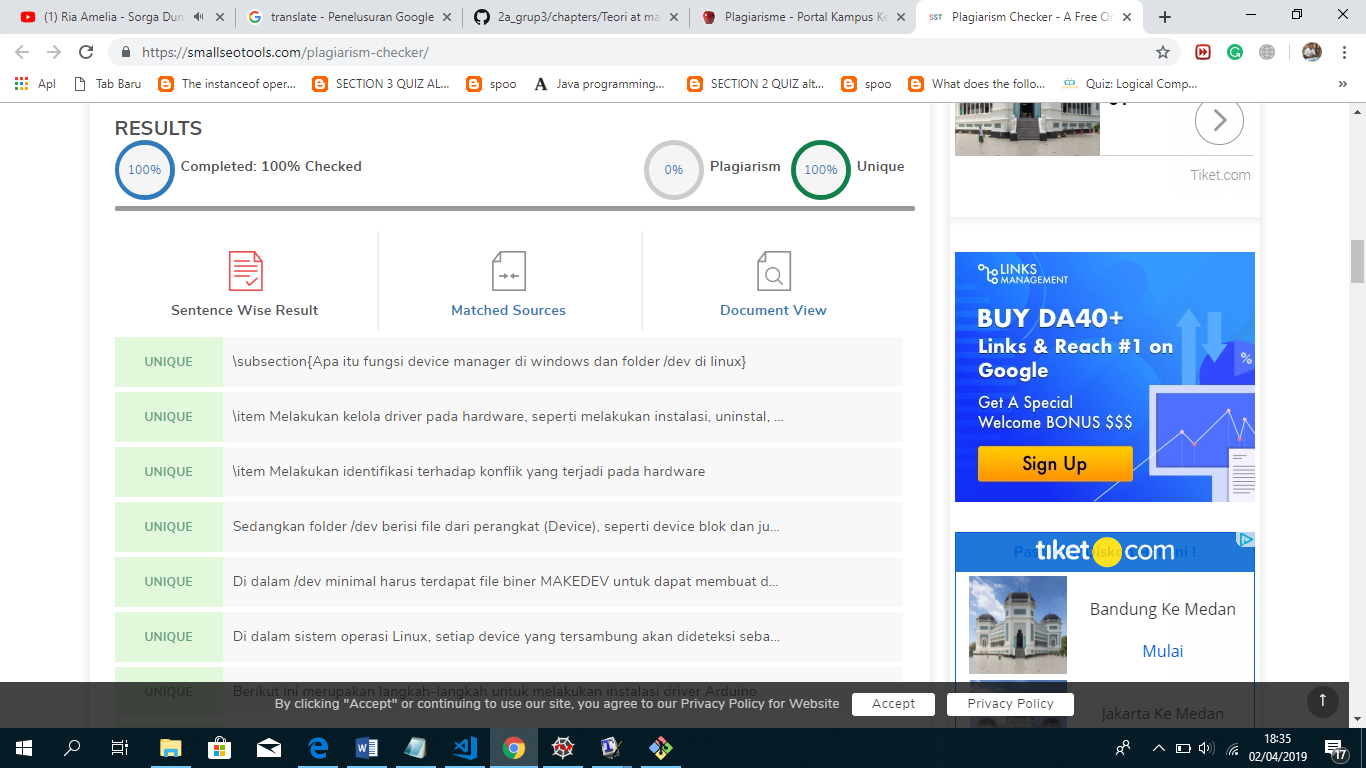
\includegraphics[scale=0.2]{figures/5/Teori/1174096/plagiat.png}
\caption{Plagiarisme}
\label{fig:plagiat}
\end{figure}

\section{Choirul Anam}
\subsection{Teori}
\subsubsection{Apa itu fungsi device manager di windows dan folder /dev di linux}
Fungsi device manager untuk membantu dan mengelola semua hardware yang terpasang dalam suatu windows.

\subsubsection{Jelaskan langkah-langkah instalasi driver dari arduino}
\begin{itemize}
    \item ubungkan sistem minimun Arduino Uno ke komputer dengan kabel USB type B (kabel Printer).
    \item Lalu pada bagian kanan didesktop PC anda, akan muncul popup “Installing device driver software”.
	\item Sistem operasi Windows tidak menyediakan driver untuk Arduino Uno, lalu proses instalasinya harus dilakukan secara manual.
	\item Buka Device Manager, caranya pada bagian Search Program and Files lalu ketikkan “device manager”.
	\item Cari Unknown device pada bagian Other device, terdapat tanda seru yang berwarna kuning, itu disebabkan karena penginstallan tidak berjalan dengan sempurna.
	\item Klik kanan pada “Unknown device”, pilih Update Driver Software.
    \item Pilih Browse my computer for driver software.
	\item Arahkan lokasi folder ke folder ..arduino-1.0.5 drivers. Pastikan check-box lalu centang include subfolders. Klik Next untuk melanjutkan instalasi driver.
	\item Kemudian lanjutkan dengan mengklik Install pada tampilan Windows Security.
	\item Jika instalasi driver berhasil maka akan muncul Windows has successfully updated your driver software.
	\item Perhatikan dan ingat nama COM Arduino Uno, karena nama COM ini yang akan digunakan untuk mengupload program nantinya.
\end{itemize}

\subsubsection{Jelaskan bagaimana cara membaca baudrate dan port dari komputer yang sudah terinstall driver}
Untuk baudrate dapat bisa dicek melalui arduino IDE, kemudian untuk mengecek port bisa dilakukan dengan device manager.

\subsubsection{Jelaskan sejarah library pyserial}
Modul ini merangkum akses untuk port serial. Ini menyediakan backends untuk Python yang berjalan di Windows, Linux, BSD (mungkin sistem yang mendukung POSIX), Jython dan IronPython (.NET dan Mono). Modul bernama "serial" secara otomatis memilih backend yang sesuai. Antarmuka berbasis kelas yang sama pada semua platform yang didukung.
Akses ke pengaturan port melalui properti Python. Dukungan untuk berbagai ukuran byte, bit stop, paritas dan kontrol aliran dengan RTS / CTS dan / atau Xon / Xoff. Bekerja dengan atau tanpa menerima batas waktu.
File seperti API dengan "read" dan "write" ("readline" dll. Juga didukung). File-file dalam paket ini adalah 100 persen Python murni. Port diatur untuk transmisi biner. Tidak ada stripping byte NULL, terjemahan CR-LF dll. (Yang berkali-kali diaktifkan untuk POSIX.) Ini membuat modul ini bermanfaat secara universal. Kompatibel dengan pustaka io (Python 2.6+)

\subsubsection{Jelaskan fungsi-fungsi apa saja yang dipakai dari library pyserial}
\begin{itemize}
    \item Serial – fungsi ini untuk membuka port serial
    \item Write(data) – untuk menulis data lewat port serial
    \item Readline() – untuk membaca string dari port serial
    \item Read(size) – untuk membaca jumlah byte dari port serial
    \item Close() – ini untuk menutup port serial 
\end{itemize}

\subsubsection{Jelaskan kenapa butuh perulangan dan tidak butuh perulangan dalam membaca serial}
Perualangan dalam bahasa pemrograman berfungsi untuk menyuruh komputer melakukan sesuatu secara berulang-ulang. Terdapat dua jenis perualangan dalam bahasa pemrograman python diantaranya adalah perulangan dengan for dan while.
Perulangan for atau counted loop (perulangan yang terhitung). Perulangan while atau uncounted loop (perulangan yang tak terhitung). Perbedaannya pada perulangan for biasanya digunakan untuk mengulangi kode yang sudah diketahui banyak perulangannya. Perualangan while untuk perulangan yang memiliki syarat dan tidak tentu berapa banyak perulangannya.
Perualangan digunakan untuk membaca data secara berulang-ulang  dan apabila tidak memakai perulangan, maka data akan terbaca satu per satu.

\subsubsection{Jelaskan bagaimana cara membuat fungsi yang mengunakan pyserial}
\lstinputlisting[firstline=8, lastline=15]{src/5/Teori/T1174004.py}

\subsection{Praktek}
\subsubsection{Kerjakan soal berikut ini, ....}
\subsubsection{Penanganan Error}

\section{Muhammad Dzihan Al-Banna}
\subsubsection{Soal 1}
Device Manager dalam system operasi Windows adalah perluasan dari Microsoft Management Console. Device Manager akan menampilkan seluruh hardware yang bisa diinisialisasi yang dikenal dengan system operasi Windows. Tampilannya terorganisir hingga dapatmemudahkan pengelolaan setiap hardware yang ada.
Fungsi-fungsi Device Manager antara lain sebagai berikut :
\begin{itemize}
\item Menunjukkan status suatu hardware
\item Menunjukkan informasi detail suatu hardware
\item Mengelola driver hardware
\item Disable \& Enable hardware
\item Meng-identifikasi konflik antar hardware, dll.
\end{itemize}
Directory pada /dev berisi file device, baik device blok maupun device karakter. di dalamnya sekurang-kurangnya  harus memiliki file biner MAKEDEV untuk membuat device ini secara manual.

\subsubsection{Soal 2}
\begin{itemize}
\item Hubungkan sistem minimun Arduino Uno ke komputer dengan kabel USB type B (kabel Printer).
\item Lalu pada bagian kanan didesktop PC anda, akan muncul popup “Installing device driver software” seperti pada gambar dibawah ini.
\item SIstem operasi Windows tidak menyediakan driver untuk Arduino Uno seperti yang terlihat pada gambar dibawah ini, lalu proses instalasinya harus dilakukan secara manual.
\item Buka Device Manager, caranya pada bagian Search Program and Files lalu ketikkan “device manager” (tanpa tanda petik), perhatikan gambar dibawah ini. Pada bagian Control Panel akan muncul Device Manager, klik untuk menjalankan.
\item Cari Unknown device pada bagian Other device, biasanya terdapat tanda seru berwarna kuning, itu disebabkan karena penginstallan tidak berjalan dengan sempurna.
\item Klik kanan pada “Unknown device” kemudian pilih Update Driver Software.
\item Pilih Browse my computer for driver software.
\item Arahkan lokasi folder ke folder arduino1.0.5 drivers. Pastikan checkbox lalu centang include subfolders. Klik Next untuk melanjutkan instalasi driver.
\item Kemudian lanjutkan dengan mengklik Install pada tampilan Windows Security.
\item Jika instalasi driver berhasil maka akan muncul Windows has successfully updated your driver software.
\item Perhatikan dan ingat nama COM Arduino Uno, karena nama COM ini yang akan digunakan untuk mengupload program nantinya.
\end{itemize}

\subsubsection{Soal 3}


Hubungkan Port USB pada Arduino dengan Port USB komputer.
Buka Software Arduino pada Komputer.
Tuliaskan program berikut ini pada Arduino Sketch.

\subsubsection{Soal 4}


Modul ini merangkum akses untuk port serial. Ini menyediakan backends untuk Python yang berjalan di Windows, Linux, BSD (mungkin sistem yang mendukung POSIX), Jython dan IronPython (.NET dan Mono). Modul bernama "serial" secara otomatis memilih backend yang sesuai. Antarmuka berbasis kelas yang sama pada semua platform yang didukung.
Akses ke pengaturan port melalui properti Python. 
Dukungan untuk berbagai ukuran byte, bit stop, paritas dan kontrol aliran dengan RTS / CTS dan / atau Xon / Xoff.
Bekerja dengan atau tanpa menerima batas waktu.
File seperti API dengan "read" dan "write" ("readline" dll. Juga didukung).
File-file dalam paket ini adalah 100 persen Phyton murni.
Port diatur untuk transmisi biner. Tidak ada stripping byte NULL, terjemahan CR-LF dll. (Yang berkali-kali diaktifkan untuk POSIX.) Ini membuat modul ini bermanfaat secara universal.
Kompatibel dengan pustaka io (Python 2.6+).

\subsubsection{Soal 5}


Fungsi-fungsi yang dipakai dari library Pyserial, diantara :
\begin{itemize}
\item Serial – fungsi ini untuk membuka port serial
\item Write(data) – untuk menulis data lewat port serial
\item Readline() – untuk membaca string dari port serial
\item Read(size) – untuk membaca jumlah byte dari port serial
\item Close() – ini untuk menutup port serial 
\end{itemize}

\subsubsection{Soal 6}


Perualangan dalam bahasa pemrograman berfungsi menyuruh komputer melakukan sesuatu secara berulang-ulang. Terdapat dua jenis perualangan dalam bahasa pemrograman python, yaitu perulangan dengan for dan while. Perulangan for disebut counted loop (perulangan yang terhitung), sementara perulangan while disebut uncounted loop (perulangan yang tak terhitung). Perbedaannya adalah perulangan for biasanya digunakan untuk mengulangi kode yang sudah diketahui banyak perulangannya. Sementara while untuk perulangan yang memiliki syarat dan tidak tentu berapa banyak perulangannya. Perulangan diperlukan agar dapat membaca data secara berulang kali sehingga data yang muncul lebih dari satu.  Sedangkan apabila tidak memakai perulangan maka data akan terbaca satu kali saja.

\subsubsection{Soal 7}


Berikut merupakan contoh penggunaan fungsi yang menggunakan pyserial
\lstinputlisting[firstline=8, lastline=15]{src/5/Teori/T1174095.py}

\subsubsection{Bukti bebas plagiarisme}
\begin{figure}[h]
\centering
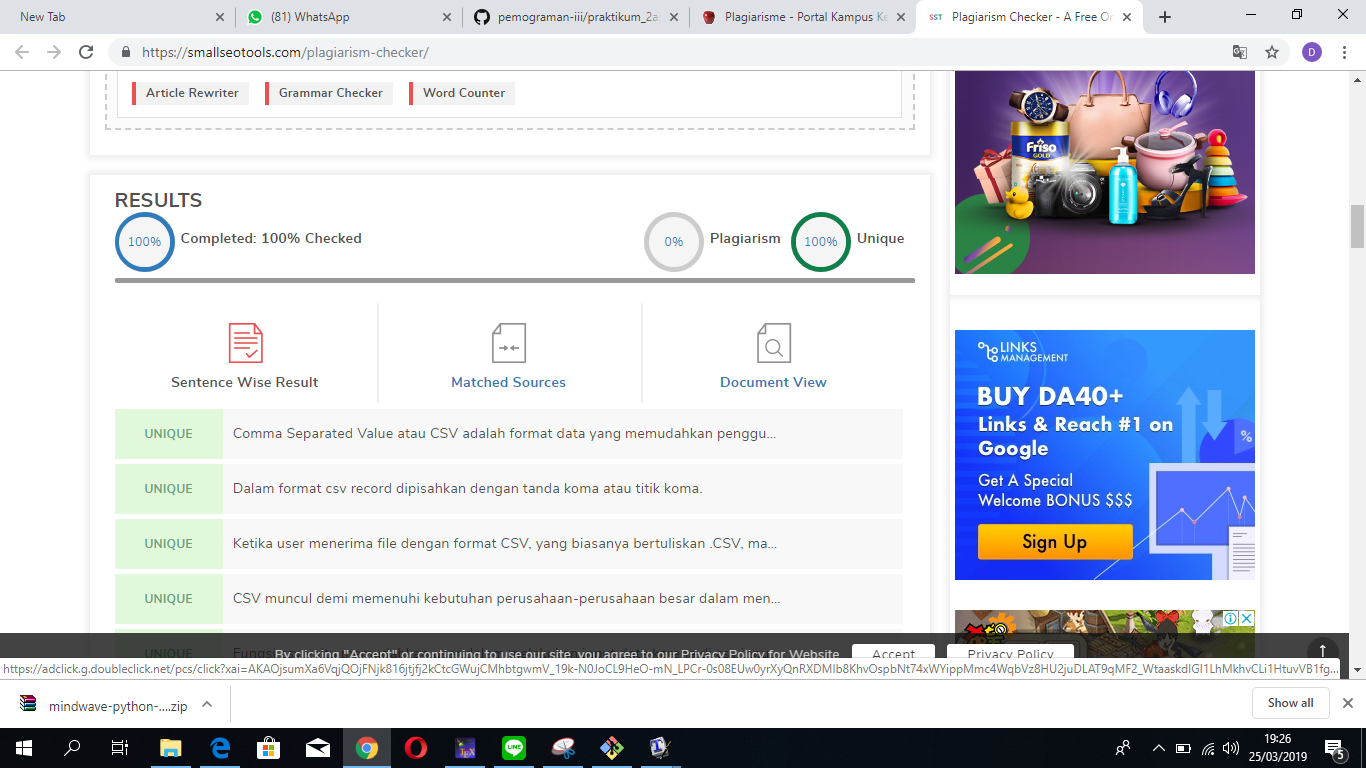
\includegraphics[width=10cm]{figures/5/Teori/1174095/1174095.png}
\caption{SS Bebas Plagiarisme}
\label{dzihan}
\end{figure}

\subsection{Praktek}
\subsubsection{Kerjakan soal berikut ini, ....}
\subsubsection{Penanganan Error}
Isi jawaban soal ke-1


%%%%%%%%%%%%%%%%%%%%%%%%%%%%%%%%%%%%%%%%%%%%%%%%%
\section{Oniwaldus Bere Mali}
\subsection{Teori}
\subsubsection{Apa itu fungsi device manager di windows dan folder /dev di linux}
Fungsi device manager dan folder /dev itu berfungsi untuk mengetahui device apa saja yang telah terinstal di leptop anda serta mengetahui port yang digunakan oleh device tersebut.

\subsubsection{Jelaskan langkah-langkah instalasi driver dari arduino}
\begin{enumerate}
\item Cara Auto
\begin{itemize}
\item Pertama Hubungkan sistem minimum Arduino Uno ke komputer dengan kabel USB type B(kabel Printer)
\begin{figure}[H] 
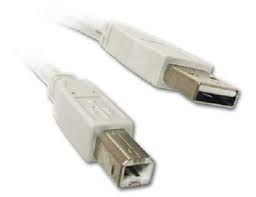
\includegraphics[width=5cm]{figures/5/Teori/1174005/1.jpg}
\centering
\caption{Membuat file csv}
\end{figure}

\item Lalu pada bagian kanan didesktop PC anda, akan muncul popup “Installing device driver software” seperti pada gambar dibawah ini.
\begin{figure}[H] 
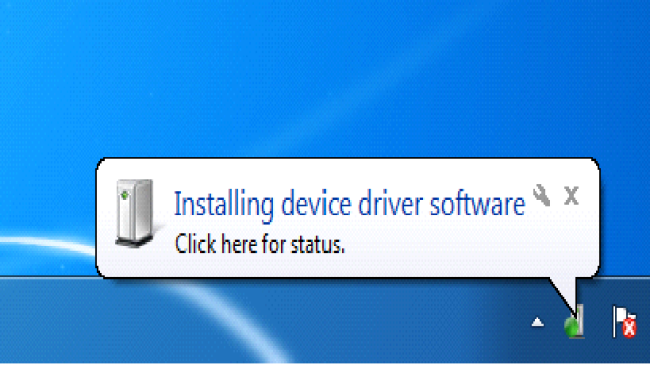
\includegraphics[width=5cm]{figures/5/Teori/1174005/2.png}
\centering
\caption{Membuat file csv}
\end{figure}

\item Tunggu hingga selesai.
\item Jika sudah selesai anda bisa mengecheck di device manager.
\begin{figure}[H] 
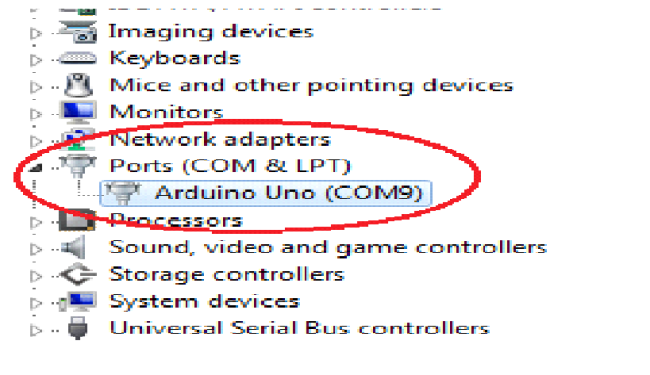
\includegraphics[width=5cm]{figures/5/Teori/1174005/11.png}
\centering
\caption{Membuat file csv}
\end{figure}
\end{itemize}

\item Cara Manual

\begin{itemize}
\item Penginstalan secara manual akan dilakukan jika penginstalan secara auto gagal dilakukan.
\item Buka Device Manager, caranya pada bagian Search Program and Files lalu ketikkan “device manager”, perhatikan gambar dibawah ini. Pada bagian Control Panel akan muncul Device Manager, klik untuk menjalankan.
\begin{figure}[H] 
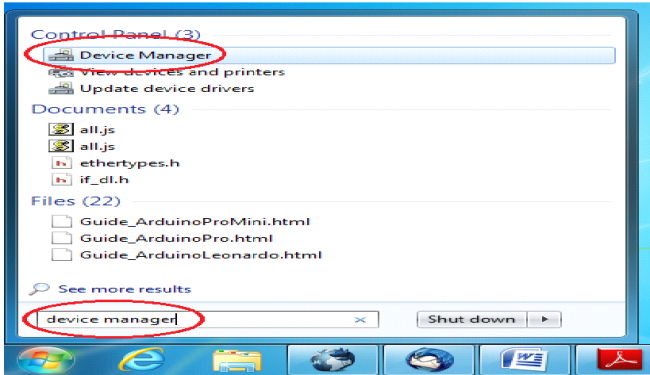
\includegraphics[width=5cm]{figures/5/Teori/1174005/4.png}
\centering
\caption{Membuat file csv}
\end{figure}

\item Cari Unknown device pada bagian Other device, biasanya terdapat tanda seru berwarna kuning, itu disebabkan karena penginstallan tidak berjalan dengan sempurna.
\begin{figure}[H] 
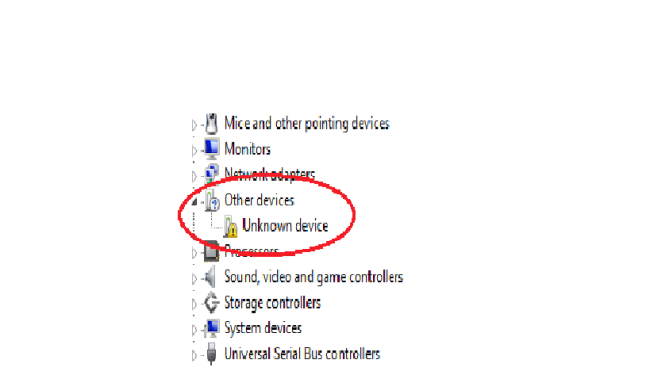
\includegraphics[width=5cm]{figures/5/Teori/1174005/5.png}
\centering
\caption{Membuat file csv}
\end{figure}

\item Klik kanan pada “Unknown device” kemudian pilih Update Driver Software.
\begin{figure}[H] 
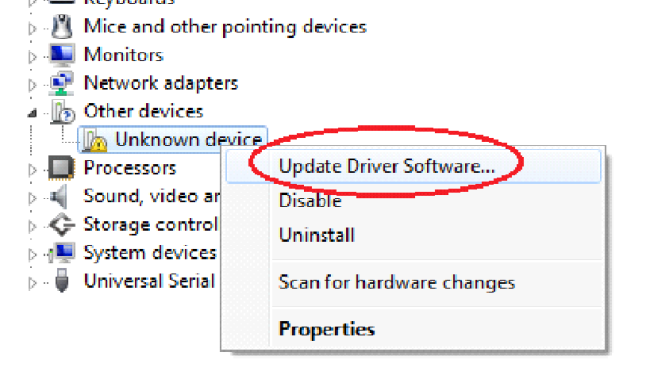
\includegraphics[width=5cm]{figures/5/Teori/1174005/6.png}
\centering
\caption{Membuat file csv}
\end{figure}

\item Pilih Browse my computer for driver software.
\begin{figure}[H] 
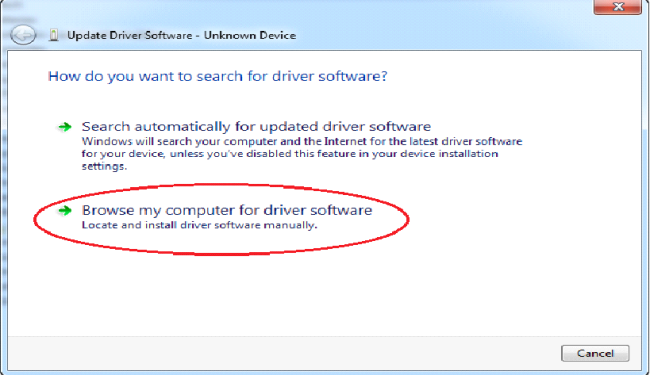
\includegraphics[width=5cm]{figures/5/Teori/1174005/7.png}
\centering
\caption{Membuat file csv}
\end{figure}

\item Arahkan lokasi folder ke folder ..arduino-1.0.5 drivers. Pastikan check-box lalu centang include subfolders. Klik Next untuk melanjutkan instalasi driver.
\begin{figure}[H] 
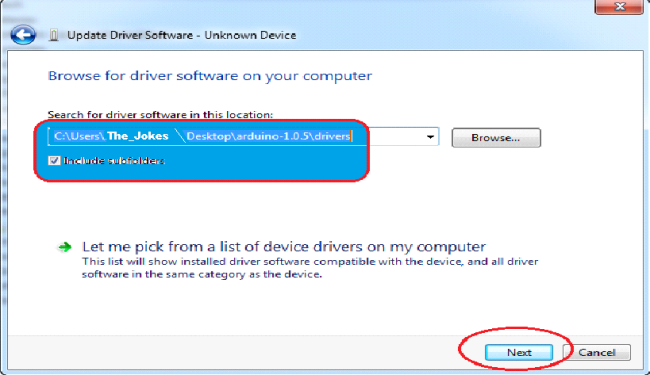
\includegraphics[width=5cm]{figures/5/Teori/1174005/8.png}
\centering
\caption{Membuat file csv}
\end{figure}

\item Kemudian lanjutkan dengan mengklik Install pada tampilan Windows Security.
\begin{figure}[H] 
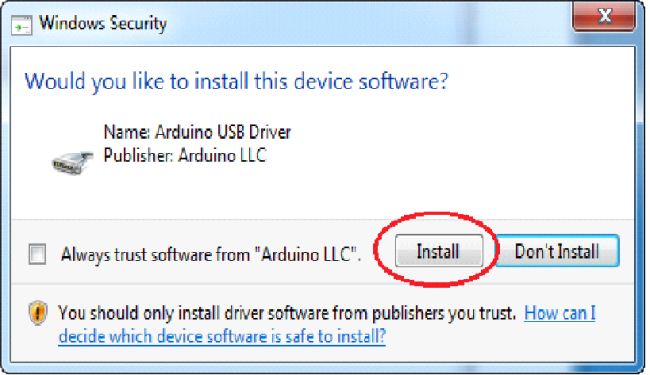
\includegraphics[width=5cm]{figures/5/Teori/1174005/9.png}
\centering
\caption{Membuat file csv}
\end{figure}

\item Jika instalasi driver berhasil maka akan muncul Windows has successfully updated your driver software.
\begin{figure}[H] 
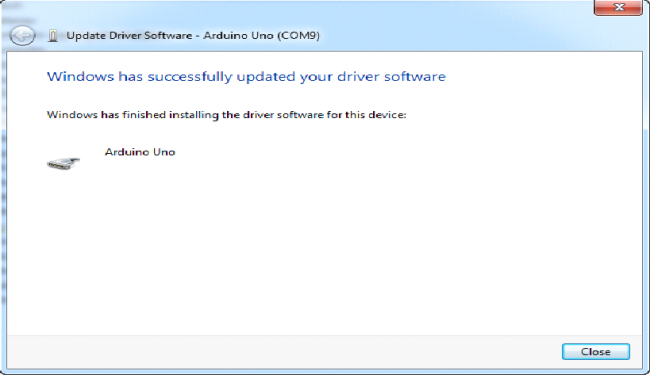
\includegraphics[width=5cm]{figures/5/Teori/1174005/10.png}
\centering
\caption{Membuat file csv}
\end{figure}

\item Perhatikan dan ingat nama COM Arduino Uno, karena nama COM ini yang akan digunakan untuk meng-upload program nantinya.
\begin{figure}[H] 
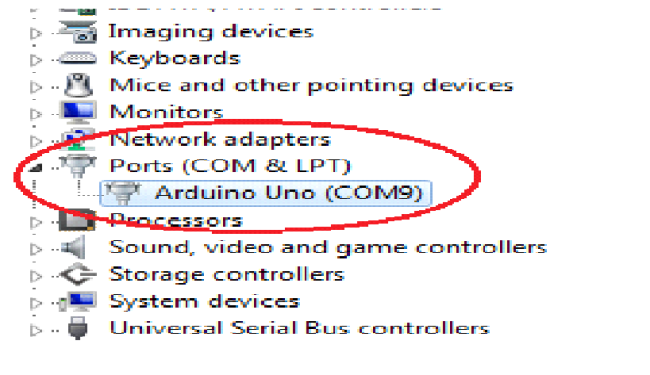
\includegraphics[width=5cm]{figures/5/Teori/1174005/11.png}
\centering
\caption{Membuat file csv}
\end{figure}
\end{itemize}
\end{enumerate}
\subsubsection{Jelaskan bagaimana cara membaca baudrate dan port dari komputer yang sudah terinstall driver}
Untuk baudrate itu bisa dicek melalui arduino IDE, kemudian untuk mengecheck port bisa dilakukan dengan device manager

\subsubsection{Jelaskan sejarah library pyserial}
Modul ini merangkum akses untuk port serial. Ini menyediakan backends untuk Python yang berjalan di Windows, Linux, BSD (mungkin sistem yang mendukung POSIX), Jython dan IronPython (.NET dan Mono). Modul bernama "serial" secara otomatis memilih backend yang sesuai. Antarmuka berbasis kelas yang sama pada semua platform yang didukung.
Akses ke pengaturan port melalui properti Python.
Dukungan untuk berbagai ukuran byte, bit stop, paritas dan kontrol aliran dengan RTS / CTS dan / atau Xon / Xoff.
Bekerja dengan atau tanpa menerima batas waktu.
File seperti API dengan "read" dan "write" ("readline" dll. Juga didukung).
File-file dalam paket ini adalah 100 persen Python murni.
Port diatur untuk transmisi biner. Tidak ada stripping byte NULL, terjemahan CR-LF dll. (Yang berkali-kali diaktifkan untuk POSIX.) Ini membuat modul ini bermanfaat secara universal.
Kompatibel dengan pustaka io (Python 2.6+)

\subsubsection{Jelaskan fungsi-fungsi apa saja yang dipakai dari library pyserial}


Serial – fungsi ini untuk membuka port serial
Write(data) – untuk menulis data lewat port serial
Readline() – untuk membaca string dari port serial
Read(size) – untuk membaca jumlah byte dari port serial
Close() – ini untuk menutup port serial 

\subsubsection{Jelaskan kenapa butuh perulangan dan tidak butuh perulangan dalam membaca serial}


Perualangan dalam bahasa pemrograman berfungsi menyuruh komputer melakukan sesuatu secara berulang-ulang. Terdapat dua jenis perualangan dalam bahasa pemrograman python, yaitu perulangan dengan for dan while.
Perulangan for disebut counted loop (perulangan yang terhitung), sementara perulangan while disebut uncounted loop (perulangan yang tak terhitung). Perbedaannya adalah perulangan for biasanya digunakan untuk mengulangi kode yang sudah diketahui banyak perulangannya. Sementara while untuk perulangan yang memiliki syarat dan tidak tentu berapa banyak perulangannya.
Perulangan diperlukan agar dapat membaca data secara berulang kali sehingga data yang muncul lebih dari satu. Sedangkan apabila tidak memakai perulangan maka data akan terbaca satu kali saja.

\subsubsection{Jelaskan bagaimana cara membuat fungsi yang mengunakan pyserial}


Berikut merupakan contoh penggunaan fungsi yang menggunakan pyserial
\lstinputlisting[firstline=8, lastline=15]{src/5/Teori/T1174005.py}

\subsubsection{Scan Plagiarisme}
\begin{figure}[H] 
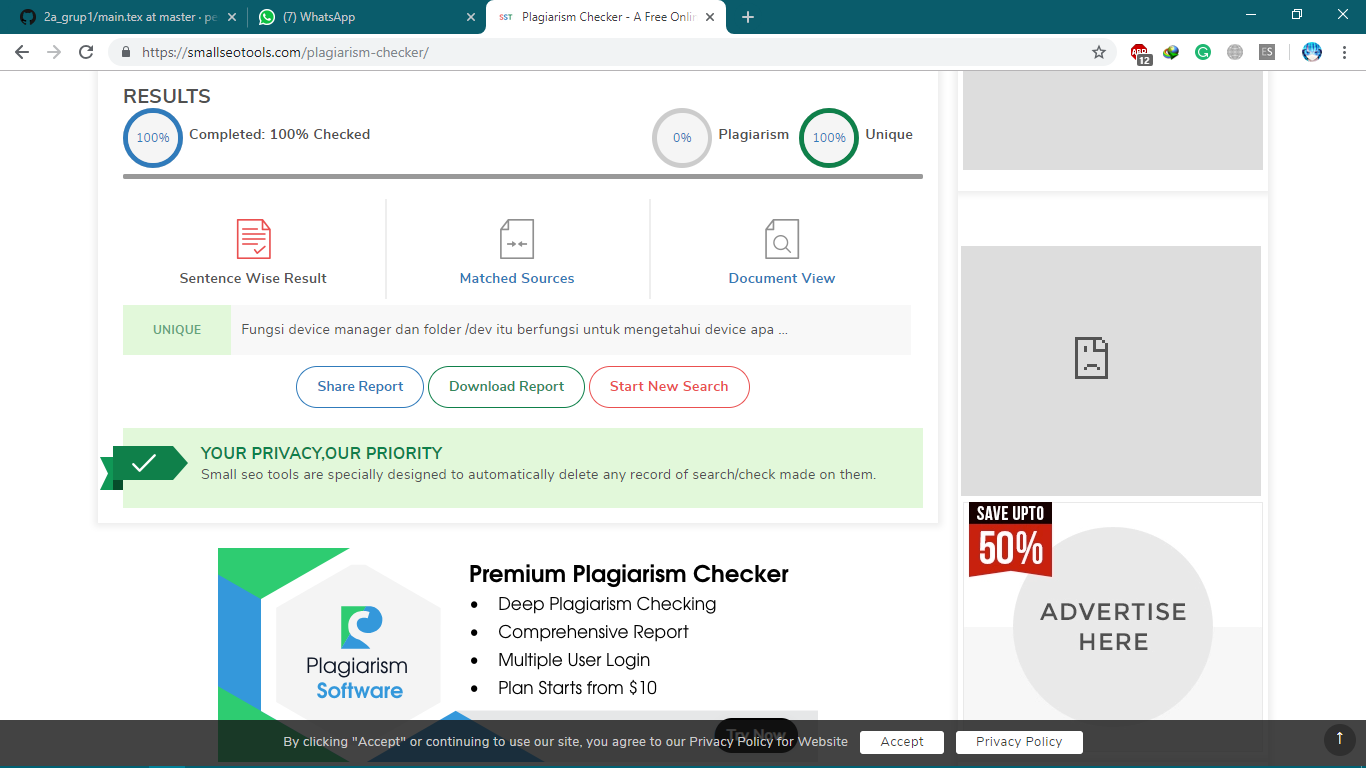
\includegraphics[width=5cm]{figures/5/Teori/1174005/nopla.png}
\centering
\caption{Membuat file csv}
\end{figure}

\subsection{Praktek}
\subsubsection{Kerjakan soal berikut ini, ....}
\subsubsection{Penanganan Error} 

%%%%%%%%%%%%%%%%%%%%%%%%%%%%%%%%%%%%%%%%%%%%%%%%%%%%%%%%%%%%%%
\section{Evietania Charis Sujadi}
{\Large \textbf{Pemahaman Teori}}
\subsection{Soal No. 1}
Apa itu fungsi device manager di windows dan folder /dev di linux?

\hfill \break
Fungsi device manager antara lain :
\begin{enumerate}
    \item Menunjukkan status suatu hardware.
    \item Menunjukkan informasi detil suatu hardware.
    \item Mengelola driver hardware
    \item Disable dan Enable hardware
    \item Mengidentifikasi konflik antar perangkat keras.
\end{enumerate}

\hfill \break
Folder /dev berisi file device, baik dari device blok maupun device karakter. Di dalamnya setidaknya ada file biner yang bernama MAKEDEV untuk membuat device secara manual.

\subsection{Soal No. 2}
Jelaskan langkah-langkah instalasi driver dari arduino!

\hfill \break
Berikut ini adalah langkah-langkah instalasi driver dari Arduino UNO di Windows:

\begin{enumerate}
    \item Hubungkan sistem minimun Arduino Uno ke komputer dengan kabel USB type B (kabel Printer).
    \item Lalu pada bagian kanan didesktop PC anda, akan muncul popup “Installing device driver software”.
    \item SIstem operasi Windows tidak menyediakan driver untuk Arduino Uno.
    \item Buka Device Manager, caranya pada bagian Search Program and Files lalu ketikkan “device manager” (tanpa tanda petik). Kemudian bagian Control Panel akan muncul halaman Device Manager, selanjutnya klik untuk menjalankan.
    \item Cari yang bernama Unknown device yang berada pada bagian Other device, biasanya ada tanda seru berwarna kuning, itu disebabkan karena penginstallan tidak berjalan dengan sempurna.
    \item Klik kanan pada “Unknown device” kemudian pilih Update Driver Software.
    \item Pilih Browse my computer for driver software.
    \item Arahkan lokasi folder ke folder ..arduino-1.0.5 drivers. Pastikan check-box lalu centang include subfolders. Klik Next untuk melanjutkan instalasi driver.
    \item Kemudian lanjutkan dengan mengklik Install pada tampilan Windows Security.
    \item Jika instalasi driver berhasil maka akan muncul Windows has successfully updated your driver software.
    \item Perhatikan dan ingat nama COM Arduino Uno, karena nama COM ini yang akan digunakan untuk meng-upload program nantinya.
\end{enumerate}

\subsection{Soal No. 3}
Jelaskan bagaimana cara membaca baudrate dan port dari komputer yang sudah terinstall driver!

\hfill \break
\textbf{Membaca Port dari Komputer}

\begin{enumerate}
    \item Hubungkan modul TX-RX serial dengan komputer melalui serial port menggunakan DB9 cable extension.
    \item Buka Hyper Terminal dengan menekan start kemudian All progams lalu Accessories kemudian Communications lalu Hyper Terminal.
    \item Ketik nama untuk Connection Description, misal coba, kemudian tekan OK.
    \item Pada Connect to, pilihlah COM port yang dipakai di Connect using, kemudian tekan OK.
    \item Masukkan nilai-nilai port settingnya, sesuai dengan DCE-nya. Kemudian tekan OK.
\end{enumerate}

\subsection{Soal No. 4}
Jelaskan sejarah library pyserial!

\hfill \break
PySerial adalah library/modul Python siap-pakai dan gratis yang dibuat untuk memudahkan kita dalam membuat program komunikasi data serial RS232 dalam bahasa Python.
Jika modul USB-2REL dapat kita kontrol dengan mudah menggunakan Python dan PyUSB, maka modul SER-2REL juga dapat kita kontrol dengan mudah menggunakan Python dengan bantuan modul PySerial.

\subsection{Soal No. 5}
Jelaskan fungsi-fungsi apa saja yang dipakai dari library pyserial!

\hfill \break
Fungsi-fungsi yang dipakai dari library PySerial, yaitu:
\begin{enumerate}
    \item Serial - fungsi ini untuk membuka port serial.
    \item write(data) - fungsi ini menulis data lewat port serial.
    \item readline() - fungsi ini membaca sebuah string dari port serial.
    \item read(size) - fungsi ini untuk membaca jumlah byte dari port serial.
    \item close() - fungsi ini untuk menutup port serial.
\end{enumerate}

\subsection{Soal No. 6}
Jelaskan kenapa butuh perulangan dan tidak butuh perulangan dalam membaca serial!

\hfill \break
Pada saat membaca serial di Arduino diperlukan perulangan agar bisa membaca data secara berulang kali sehingga data yang muncul banyak. Sedangkan apabila tidak membutuhkan perulangan maka Arduino hanya akan membaca data sekali saja.

\subsection{Soal No. 7}
Jelaskan bagaimana cara membuat fungsi yang mengunakan pyserial!

\hfill \break
Fungsi yang berada pada Python, dibuat dengan nama kata kunci def kemudian diikuti dengan nama fungsinya pada pyhton.
Seperti halnya dengan blok kode yang lain, kita juga harus memberikan identasi untuk menuliskan isi fungsi.

\subsubsection{Bukti bebas plagiarisme}
\begin{figure}[h]
\centering
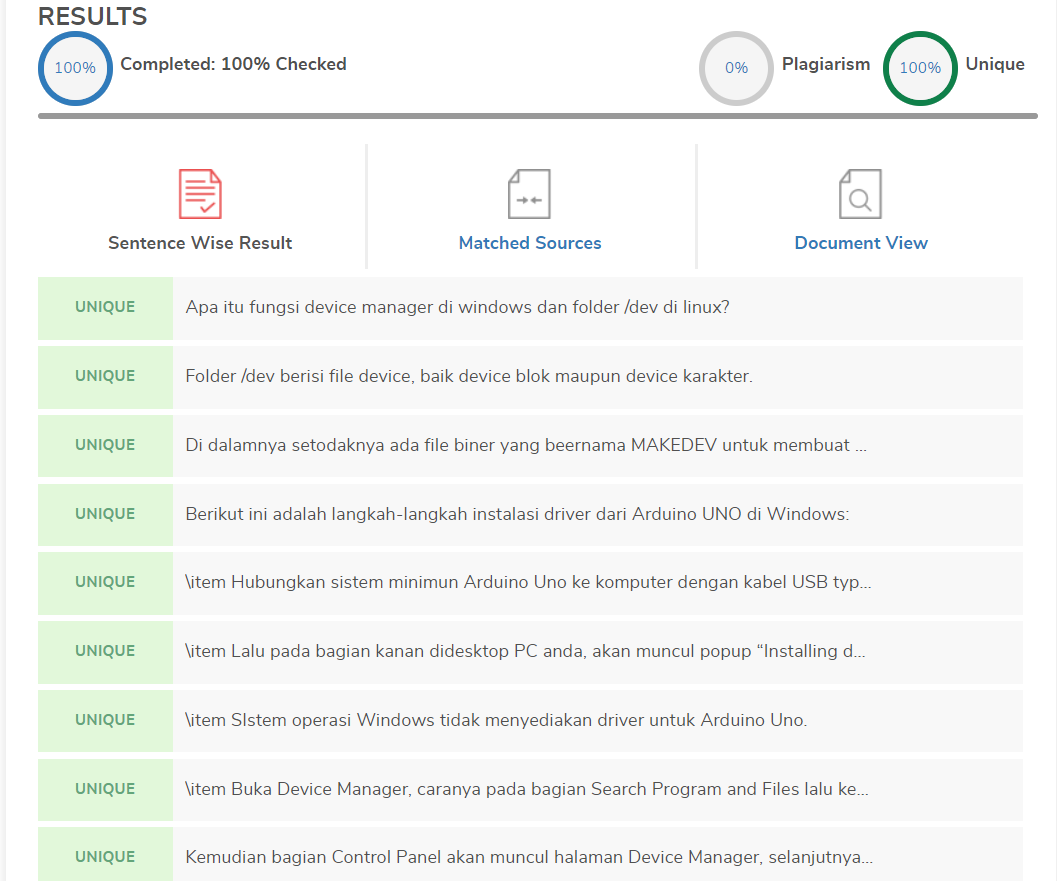
\includegraphics[width=10cm]{figures/5/Teori/1174051/Plagiat.png}
\caption{Bebas Plagiarisme}
\label{Evietania}
\end{figure}

%%%%%%%%%%%%%%%%%%%%%%%%%%%%%%%%%%%%%%%%%%%%%%%%%%%%%%%%%%%%%%%%%%%

\section{Dezha Aidil Martha}
\subsection{Bagian 1 - Teori}
\subsubsection{Apa itu fungsi device manager di windows dan folder /dev di linux}
Fungsi device manager dan folder /dev itu berfungsi untuk mengetahui device apa saja yang telah terinstal di leptop anda serta mengetahui port yang digunakan oleh device tersebut.

\subsubsection{Jelaskan langkah-langkah instalasi driver dari arduino}
\begin{enumerate}
\item Cara Auto
\begin{itemize}
\item Pertama Hubungkan sistem minimum Arduino Uno ke komputer dengan kabel USB type B(kabel Printer)
\begin{figure}[H] 
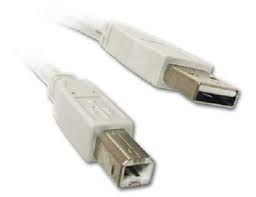
\includegraphics[width=5cm]{figures/5/Teori/1174025/no1.jpg}
\centering
\caption{Koneksikan Arduino Uno menggunakan kabel}
\end{figure}

\item Lalu pada bagian kanan didesktop PC anda, akan muncul popup “Installing device driver software” seperti pada gambar dibawah ini.
\begin{figure}[H] 
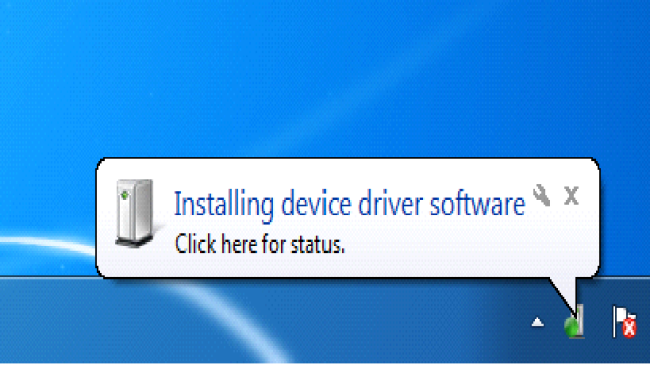
\includegraphics[width=5cm]{figures/5/Teori/1174025/no2.png}
\centering
\end{figure}

\item Tunggu hingga selesai.
\item Jika sudah selesai anda bisa mengecheck di device manager.
\begin{figure}[H] 
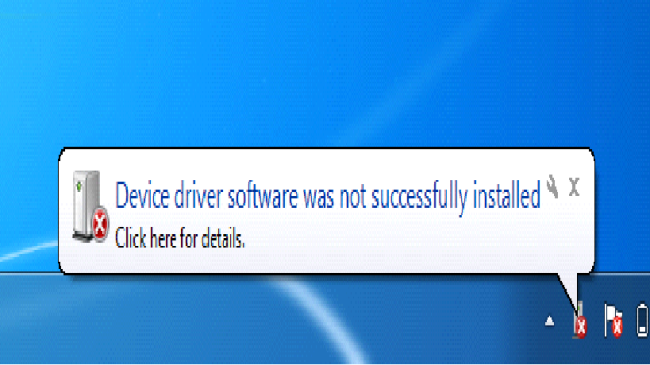
\includegraphics[width=5cm]{figures/5/Teori/1174025/no3.png}
\centering
\caption{Cek driver sudah terinstall atau belum}
\end{figure}
\end{itemize}

\item Cara Manual
\begin{itemize}
\item Penginstalan secara manual akan dilakukan jika penginstalan secara auto gagal dilakukan.
\item Buka Device Manager, caranya pada bagian Search Program and Files lalu ketikkan “device manager”, perhatikan gambar dibawah ini. Di bagian Control Panel akan muncul Device Manager, klik untuk menjalankan.
\begin{figure}[H] 
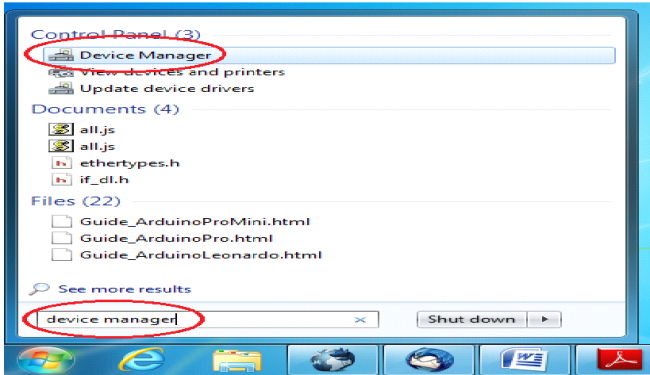
\includegraphics[width=5cm]{figures/5/Teori/1174025/no4.png}
\centering
\caption{Instalasi driver secara manual}
\end{figure}

\item Cari Unknown device pada bagian Other device, pada umumnya terdapat tanda seru berwarna kuning, itu disebabkan karena penginstallan tidak berjalan dengan lancar.
\begin{figure}[H] 
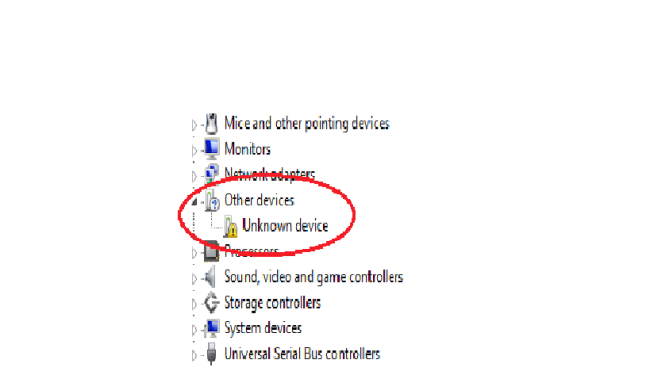
\includegraphics[width=5cm]{figures/5/Teori/1174025/no5.png}
\centering
\end{figure}

\item Klik kanan pada “Unknown device” kemudian pilih Update Driver Software.
\begin{figure}[H] 
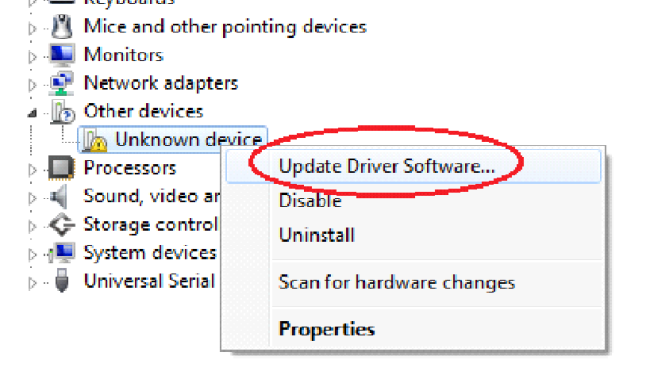
\includegraphics[width=5cm]{figures/5/Teori/1174025/no6.png}
\centering
\end{figure}

\item Lalu Pilih Browse my computer for driver software.
\begin{figure}[H] 
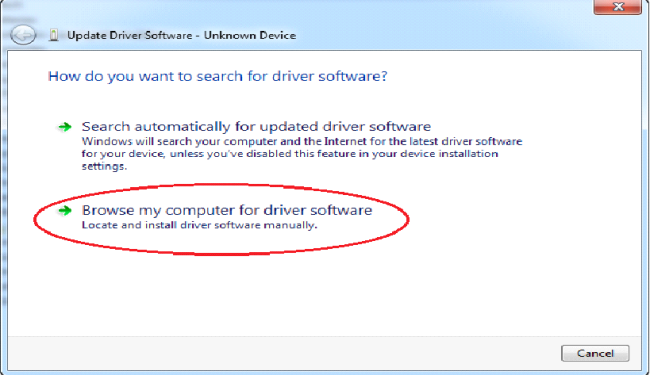
\includegraphics[width=5cm]{figures/5/Teori/1174025/no7.png}
\centering
\end{figure}

\item Arahkan lokasi folder ke folder ..arduino-1.0.5 drivers. Pastikan check-box lalu centang include subfolders. Klik Next untuk melanjutkan instalasi driver.
\begin{figure}[H] 
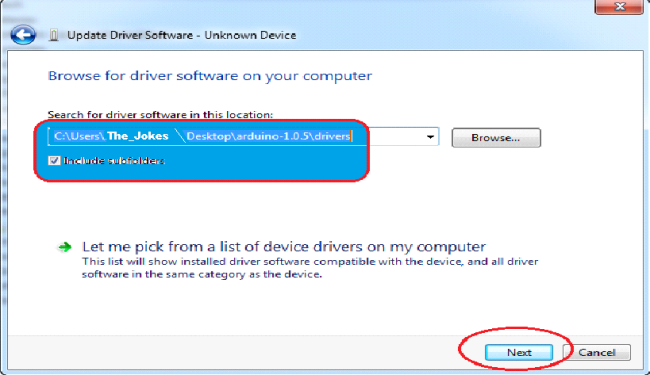
\includegraphics[width=5cm]{figures/5/Teori/1174025/no8.png}
\centering
\end{figure}

\item Kemudian lanjutkan dengan mengklik Install pada tampilan Windows Security.
\begin{figure}[H] 
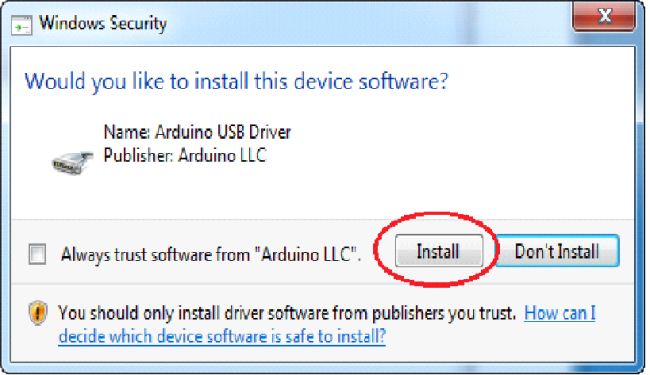
\includegraphics[width=5cm]{figures/5/Teori/1174025/no9.png}
\centering
\end{figure}

\item Jika instalasi driver berhasil maka akan muncul Windows has successfully updated your driver software.
\begin{figure}[H] 
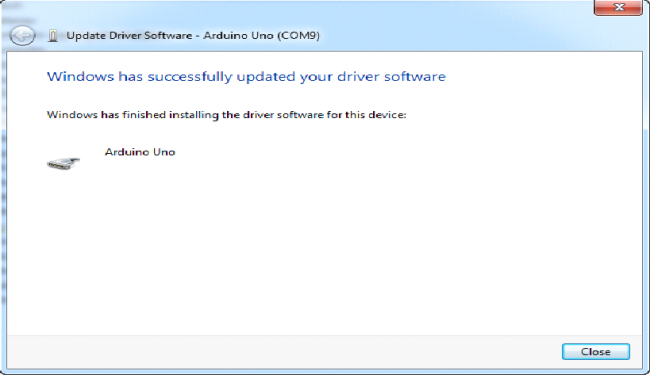
\includegraphics[width=5cm]{figures/5/Teori/1174025/no10.png}
\centering
\end{figure}

\item Perhatikan dan ingat nama COM Arduino Uno, karena nama COM ini yang akan digunakan untuk meng-upload program nantinya.
\begin{figure}[H] 
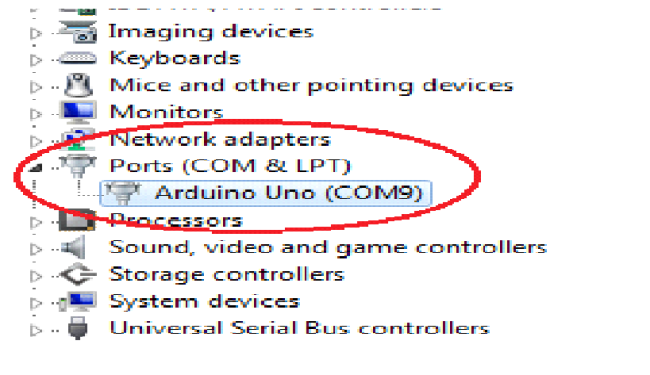
\includegraphics[width=5cm]{figures/5/Teori/1174025/no11.png}
\centering
\end{figure}
\end{itemize}
\end{enumerate}
\subsubsection{Jelaskan bagaimana cara membaca baudrate dan port dari komputer yang sudah terinstall driver}
Untuk baudrate itu bisa dicek melalui arduino IDE, kemudian untuk mengecheck port bisa dilakukan dengan device manager

\subsubsection{Jelaskan sejarah library pyserial}
Modul ini merangkum akses untuk port serial. Ini menyediakan backends untuk Python yang berjalan di Windows, Linux, BSD (mungkin sistem yang mendukung POSIX), Jython dan IronPython (.NET dan Mono). Modul bernama "serial" secara otomatis memilih backend yang sesuai. Antarmuka berbasis kelas yang sama pada semua platform yang didukung.
Akses ke pengaturan port melalui properti Python.
Dukungan untuk berbagai ukuran byte, bit stop, paritas dan kontrol aliran dengan RTS / CTS dan / atau Xon / Xoff.
Bekerja dengan atau tanpa menerima batas waktu.
File seperti API dengan "read" dan "write" ("readline" dll. Juga didukung).
File-file dalam paket ini adalah 100 persen Python murni.
Port diatur untuk transmisi biner. Tidak ada stripping byte NULL, terjemahan CR-LF dll. (Yang berkali-kali diaktifkan untuk POSIX.) Ini membuat modul ini bermanfaat secara universal.
Kompatibel dengan pustaka io (Python 2.6+)

\subsubsection{Jelaskan fungsi-fungsi apa saja yang dipakai dari library pyserial}


Serial – fungsi ini untuk membuka port serial
Write(data) – untuk menulis data lewat port serial
Readline() – untuk membaca string dari port serial
Read(size) – untuk membaca jumlah byte dari port serial
Close() – ini untuk menutup port serial 

\subsubsection{Jelaskan kenapa butuh perulangan dan tidak butuh perulangan dalam membaca serial}


Perualangan dalam bahasa pemrograman berfungsi menyuruh komputer melakukan sesuatu secara berulang-ulang. Terdapat dua jenis perualangan dalam bahasa pemrograman python, yaitu perulangan dengan for dan while.
Perulangan for disebut counted loop (perulangan yang terhitung), sementara perulangan while disebut uncounted loop (perulangan yang tak terhitung). Perbedaannya ialah, perulangan (for) biasanya dipakai untuk mengulangi kode yang sudah diketahui banyak perulangannya. Sementara itu, perulangan (while) dipakai untuk perulangan yang memiliki syarat dan tidak tentu berapa banyak perulangannya.
Perulangan diperlukan agar dapat membaca data secara berulang kali sehingga data yang muncul lebih dari satu. Sedangkan apabila tidak memakai perulangan maka data akan terbaca satu kali saja.

\subsubsection{Jelaskan bagaimana cara membuat fungsi yang mengunakan pyserial}


Berikut merupakan contoh penggunaan fungsi yang menggunakan pyserial
\lstinputlisting[firstline=8, lastline=15]{src/5/Teori/T1174025.py}

\subsubsection{Scan Plagiarisme}
\begin{figure}[H] 
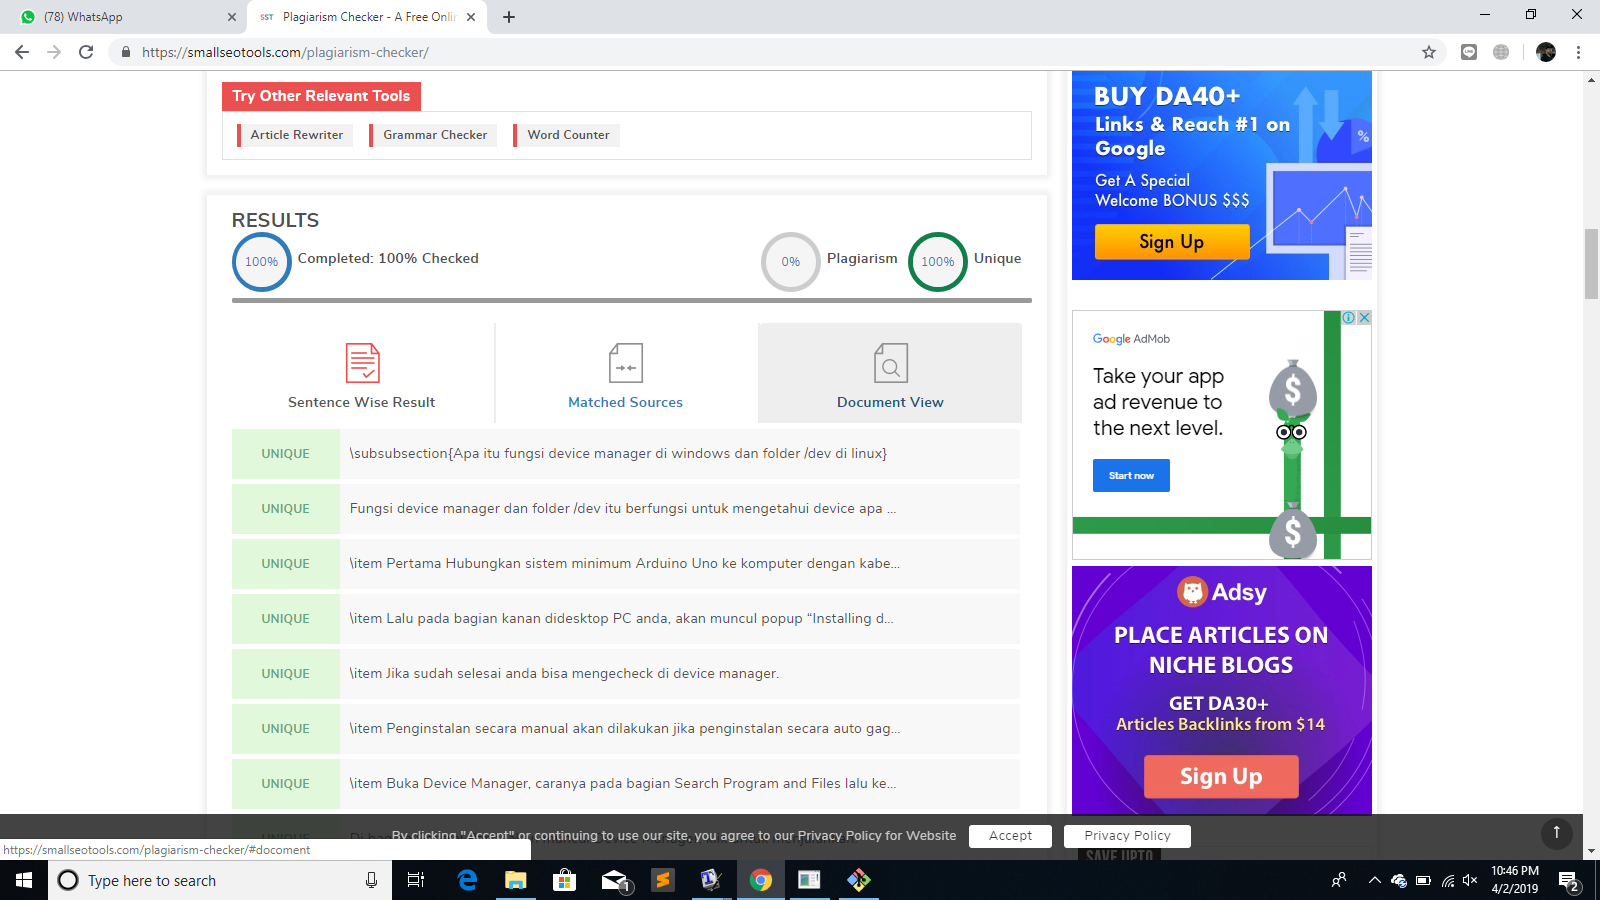
\includegraphics[width=5cm]{figures/5/Teori/1174025/noplg.png}
\centering
\end{figure}